% !TEX Root = ../proposal.tex

% slides discussing variational integrator
\section*{}
\subsection*{Variational Integrator}
\begin{frame} %------------------------------------%
\frametitle{Variational Principle}
    \begin{itemize}
        \item Variational Integrators
            \begin{itemize}
                \item Structure-preserving integrators for Hamiltonian systems
                \item Obtained by discretizing variational principle
            \end{itemize}
    \end{itemize}
    \pause
    \begin{columns}[c]
        \begin{column}{0.5\textwidth}
            \centering
            \begin{beamercolorbox}[wd=0.8\columnwidth,sep=0.05cm,center]{numerical} Continuous Time \end{beamercolorbox}
            \begin{beamercolorbox}[wd=0.8\columnwidth,sep=0.05cm,center]{numerical} 
                Configuration Space \\
                \( \parenth{q, \dot{q} } \in TQ \)
            \end{beamercolorbox}
            \begin{beamercolorbox}[wd=0.8\columnwidth,sep=0.05cm,center]{numerical} 
                Lagrangian \\
                \( L\parenth{q, \dot{q} } \)
            \end{beamercolorbox}
            \begin{beamercolorbox}[wd=0.8\columnwidth,sep=0.05cm,center]{numerical} 
                Action Integral \\
                \( S = \int_{0}^T L\left( q, \dot{q}\right) \, dt \)
            \end{beamercolorbox}
            \begin{beamercolorbox}[wd=0.8\columnwidth,sep=0.05cm,center]{numerical} 
                Stationary Action \\
                \( \delta S = 0 \)
            \end{beamercolorbox}
%           \begin{beamercolorbox}[wd=0.8\columnwidth,sep=0.05cm,center]{numerical} 
%               Legendre Transform \\
%               \( p_i = \deriv{L}{\dot{q}} \)
%           \end{beamercolorbox}
            \begin{beamercolorbox}[wd=0.8\columnwidth,sep=0.05cm,center]{numerical} 
                Equation of Motion \\
                \( \ddot{q} = f \parenth{q, \dot{q} } \)
            \end{beamercolorbox}
        \end{column}
        \pause
        \begin{column}{0.5\textwidth}
            \centering
            \begin{beamercolorbox}[wd=0.8\columnwidth,sep=0.05cm,center]{numerical} Discrete Time \end{beamercolorbox}
            \begin{beamercolorbox}[wd=0.8\columnwidth,sep=0.05cm,center]{numerical} 
                Configuration Space \\
                \( \parenth{q_k, q_{k+1} } \in Q \times Q \)
            \end{beamercolorbox}
            \begin{beamercolorbox}[wd=0.8\columnwidth,sep=0.05cm,center]{numerical} 
                Lagrangian \\
                \( L_d\parenth{q_k, q_{k+1}} \)
            \end{beamercolorbox}
            \begin{beamercolorbox}[wd=0.8\columnwidth,sep=0.05cm,center]{numerical} 
                Action Sum \\
                \( S_d = \sum_{k=0}^{N-1} L_d(q_k, q_{k+1}) \)
            \end{beamercolorbox}
            \begin{beamercolorbox}[wd=0.8\columnwidth,sep=0.05cm,center]{numerical} 
                Stationary Action \\
                \( \delta S_d = 0 \)
            \end{beamercolorbox}
%           \begin{beamercolorbox}[wd=0.8\columnwidth,sep=0.05cm,center]{numerical} 
%               Fiber Derivative \\
%               \( p_k = - \deriv{L_d(q_k, q_{k+1})}{q_k} \) \\
%               \( p_{k+1} = \deriv{L_d(q_k, q_{k+1})}{q_{k+1}} \)
%           \end{beamercolorbox}
            \begin{beamercolorbox}[wd=0.8\columnwidth,sep=0.05cm,center]{numerical} 
                Equation of Motion \\
                \( q_{k+2} = f_d \parenth{q_k, q_{k+1} } \)
            \end{beamercolorbox}
        \end{column}
    \end{columns}
    
    \note[itemize]{
        \item Continous time - discretization occurs at end while implemented in digital computer
        \item Discrete time - discretization occurs at the beginning. 
        Dynamics derived in discrete time
        \item Legendre transform allows for expression of dynamics in Hamiltonian form
    }
\end{frame}%-----------------------------------------%

\begin{frame}[shrink=20] %------------------------------------------%
\frametitle{Discrete Lagrangian}
    Continuous time Lagrangian
    \begin{align*}
        L = \frac{1}{2} \left( \left( \dot{x} -y \right)^2 + \left( \dot{y} + x \right)^2 \right) + \frac{1-\mu}{r_1} + \frac{\mu}{r_2}
    \end{align*}
    Choice of Quadrature rule affects accuracy
    \begin{table}[htbp]
        \centering
        \begin{tabular}{l|l}Rectangle & \( L_d(q_0,q_1) =L(q_0,\frac{q_1-q_0}{h}) h \)  \\ \hline \hline
        Midpoint & \( L_d(q_0,q_1) = L(\frac{q_0 + q_1}{2},\frac{q_1 - q_0}{h}) h \) \\ \hline \hline
        Trapezoidal & \( L_d(q_0, q_1) = \frac{1}{2} \left[ L(q_0, \frac{q_1 - q_0}{h} ) + L(q_1, \frac{q_1 - q_0 }{h} )\right] h \)
        \end{tabular} 
    \end{table}
    Discrete time Lagrangian using Trapezoidal Rule
    \begin{align*}
        L_d &= \frac{h}{2} \left( \frac{1}{2} \bracket{\left(  \frac{\xkp - \xk}{h} -\yk \right)^2 + \left( \frac{\ykp - \yk}{h} + \xk \right)^2} + \frac{1 - \mu}{r_{1_k}} + \frac{\mu}{r_{2_k}} \right. \nonumber \\ 
    &+ \left. \frac{1}{2} \bracket{\left(  \frac{\xkp - \xk}{h} -\ykp \right)^2 + \left( \frac{\ykp - \yk}{h} + \xkp \right)^2} + \frac{1-\mu}{r_{1_{k+1}}} + \frac{\mu}{r_{2_{k+1}}}  \right)
    \end{align*}
    
    \note[itemize]{
        \item Apply E-L equations to discrete time Lagrangian to get discrete EOMs
    }
\end{frame} %--------------------------------------------%

\begin{frame}[t] %---------------------------------------------------%
\frametitle{Integrator Comparison}
    \begin{itemize}
        \item Numerical Simulation of PCRTBP (\( t_f = 200 \approx 15 \) years)
            \begin{itemize}
                \item Variable step Runge-Kutta method (\texttt{ode45.m})
                \item Variational integrator \( \bar{x}_k \to \bar{x}_{k+1} \)
            \end{itemize} 
    \end{itemize}
    \begin{figure} 
    \centering 
        \visible<2->{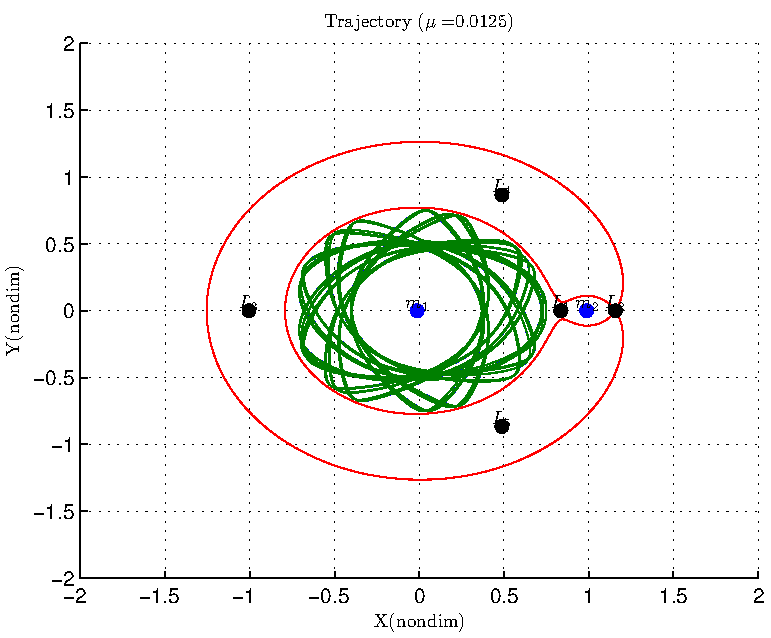
\includegraphics[width=0.5\textwidth]{./integrator_compare/trajectory}}% 
        \visible<2->{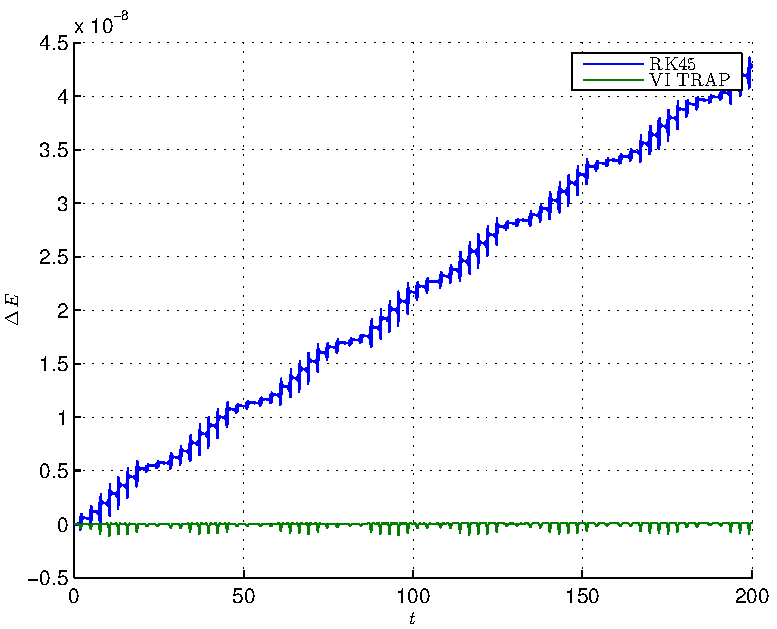
\includegraphics[width=0.5\textwidth]{./integrator_compare/energy} }
    \end{figure}
    
    \begin{itemize}
        \visible<2->{\item Typical integration methods do not preserve structure}
    \end{itemize}
\end{frame} %------------------------------------------------------%